
%-----------------------------------------------------------------------------------------------------------------------------------------------%
%	The MIT License (MIT)
%
%	Copyright (c) 2021 Philip Empl
%
%	Permission is hereby granted, free of charge, to any person obtaining a copy
%	of this software and associated documentation files (the "Software"), to deal
%	in the Software without restriction, including without limitation the rights
%	to use, copy, modify, merge, publish, distribute, sublicense, and/or sell
%	copies of the Software, and to permit persons to whom the Software is
%	furnished to do so, subject to the following conditions:
%	
%	THE SOFTWARE IS PROVIDED "AS IS", WITHOUT WARRANTY OF ANY KIND, EXPRESS OR
%	IMPLIED, INCLUDING BUT NOT LIMITED TO THE WARRANTIES OF MERCHANTABILITY,
%	FITNESS FOR A PARTICULAR PURPOSE AND NONINFRINGEMENT. IN NO EVENT SHALL THE
%	AUTHORS OR COPYRIGHT HOLDERS BE LIABLE FOR ANY CLAIM, DAMAGES OR OTHER
%	LIABILITY, WHETHER IN AN ACTION OF CONTRACT, TORT OR OTHERWISE, ARISING FROM,
%	OUT OF OR IN CONNECTION WITH THE SOFTWARE OR THE USE OR OTHER DEALINGS IN
%	THE SOFTWARE.
%	
%
%-----------------------------------------------------------------------------------------------------------------------------------------------%


%============================================================================%
%
%	DOCUMENT DEFINITION
%
%============================================================================%

\documentclass[10pt,A4,english]{article}	


%----------------------------------------------------------------------------------------
%	ENCODING
%----------------------------------------------------------------------------------------

% we use utf8 since we want to build from any machine
\usepackage[utf8]{inputenc}		
\usepackage[USenglish]{isodate}
\usepackage{fancyhdr}
\usepackage[numbers]{natbib}

%----------------------------------------------------------------------------------------
%	LOGIC
%----------------------------------------------------------------------------------------

% provides \isempty test
\usepackage{xstring, xifthen}
\usepackage{enumitem}
\usepackage[english]{babel}
\usepackage{blindtext}
\usepackage{pdfpages}
\usepackage{changepage}
%----------------------------------------------------------------------------------------
%	FONT BASICS
%----------------------------------------------------------------------------------------

% some tex-live fonts - choose your own

% \usepackage[defaultsans]{droidsans}
%\usepackage[default]{comfortaa}
%\usepackage{cmbright}
\usepackage[default]{raleway}
% \usepackage{fetamont}
%\usepackage[default]{gillius}
%\usepackage[light,math]{iwona}
% \usepackage[thin]{roboto}

% set font default
\renewcommand*\familydefault{\sfdefault} 	
\usepackage[T1]{fontenc}

% more font size definitions
\usepackage{moresize}

%----------------------------------------------------------------------------------------
%	FONT AWESOME ICONS
%---------------------------------------------------------------------------------------- 

% include the fontawesome icon set
\usepackage{fontawesome}

% use to vertically center content
% credits to: http://tex.stackexchange.com/questions/7219/how-to-vertically-center-two-images-next-to-each-other
\newcommand{\vcenteredinclude}[1]{\begingroup
\setbox0=\hbox{\includegraphics{#1}}%
\parbox{\wd0}{\box0}\endgroup}
\newcommand{\tab}[1]{\hspace{.2\textwidth}\rlap{#1}}
% use to vertically center content
% credits to: http://tex.stackexchange.com/questions/7219/how-to-vertically-center-two-images-next-to-each-other
\newcommand*{\vcenteredhbox}[1]{\begingroup
\setbox0=\hbox{#1}\parbox{\wd0}{\box0}\endgroup}

% icon shortcut
\newcommand{\icon}[3] { 							
	\makebox(#2, #2){\textcolor{maincol}{\csname fa#1\endcsname}}
}	


% icon with text shortcut
\newcommand{\icontext}[4]{ 						
	\vcenteredhbox{\icon{#1}{#2}{#3}}  \hspace{2pt}  \parbox{0.9\mpwidth}{\textcolor{#4}{#3}}
}

% icon with website url
\newcommand{\iconhref}[5]{ 						
    \vcenteredhbox{\icon{#1}{#2}{#5}}  \hspace{2pt} \href{#4}{\textcolor{#5}{#3}}
}

% icon with email link
\newcommand{\iconemail}[5]{ 						
    \vcenteredhbox{\icon{#1}{#2}{#5}}  \hspace{2pt} \href{mailto:#4}{\textcolor{#5}{#3}}
}

%----------------------------------------------------------------------------------------
%	PAGE LAYOUT  DEFINITIONS
%----------------------------------------------------------------------------------------

% page outer frames (debug-only)
% \usepackage{showframe}		

% we use paracol to display breakable two columns
\usepackage{paracol}
\usepackage{tikzpagenodes}
\usetikzlibrary{calc}
\usepackage{lmodern}
\usepackage{multicol}
\usepackage{lipsum}
\usepackage{atbegshi}
% define page styles using geometry
\usepackage[a4paper]{geometry}

% remove all possible margins
\geometry{top=1cm, bottom=1cm, left=1cm, right=1cm}

\usepackage{fancyhdr}
\pagestyle{empty}

% space between header and content
% \setlength{\headheight}{0pt}

% indentation is zero
\setlength{\parindent}{0mm}

%----------------------------------------------------------------------------------------
%	TABLE /ARRAY DEFINITIONS
%---------------------------------------------------------------------------------------- 

% extended aligning of tabular cells
\usepackage{array}

% custom column right-align with fixed width
% use like p{size} but via x{size}
\newcolumntype{x}[1]{%
>{\raggedleft\hspace{0pt}}p{#1}}%


%----------------------------------------------------------------------------------------
%	GRAPHICS DEFINITIONS
%---------------------------------------------------------------------------------------- 

%for header image
\usepackage{graphicx}

% use this for floating figures
% \usepackage{wrapfig}
% \usepackage{float}
% \floatstyle{boxed} 
% \restylefloat{figure}

%for drawing graphics		
\usepackage{tikz}			
\usepackage{ragged2e}	
\usetikzlibrary{shapes, backgrounds,mindmap, trees}

%----------------------------------------------------------------------------------------
%	Color DEFINITIONS
%---------------------------------------------------------------------------------------- 
\usepackage{transparent}
\usepackage{color}

% primary color
\definecolor{maincol}{RGB}{64,64,64}

% accent color, secondary
% \definecolor{accentcol}{RGB}{ 250, 150, 10 }

% dark color
\definecolor{darkcol}{RGB}{70,70,70}

% light color
\definecolor{lightcol}{RGB}{245,245,245}

\definecolor{accentcol}{RGB}{59,77,97}



% Package for links, must be the last package used
\usepackage[hidelinks]{hyperref}

% returns minipage width minus two times \fboxsep
% to keep padding included in width calculations
% can also be used for other boxes / environments
\newcommand{\mpwidth}{\linewidth-\fboxsep-\fboxsep}
	


%============================================================================%
%
%	CV COMMANDS
%
%============================================================================%

%----------------------------------------------------------------------------------------
%	 CV LIST
%----------------------------------------------------------------------------------------

% renders a standard latex list but abstracts away the environment definition (begin/end)
\newcommand{\cvlist}[1] {
	\begin{itemize}{#1}\end{itemize}
}

%----------------------------------------------------------------------------------------
%	 CV TEXT
%----------------------------------------------------------------------------------------

% base class to wrap any text based stuff here. Renders like a paragraph.
% Allows complex commands to be passed, too.
% param 1: *any
\newcommand{\cvtext}[1] {
	\begin{tabular*}{1\mpwidth}{p{0.98\mpwidth}}
		\parbox{1\mpwidth}{#1}
	\end{tabular*}
}
\newcommand{\cvtextsmall}[1] {
	\begin{tabular*}{0.8\mpwidth}{p{0.8\mpwidth}}
		\parbox{0.8\mpwidth}{#1}
	\end{tabular*}
}
%----------------------------------------------------------------------------------------
%	CV SECTION
%----------------------------------------------------------------------------------------

% Renders a a CV section headline with a nice underline in main color.
% param 1: section title
\newcommand{\cvsection}[1] {
	\vspace{14pt}
	\cvtext{
		\textbf{\LARGE{\textcolor{darkcol}{#1}}}\\[-4pt]
		\textcolor{accentcol}{ \rule{0.2\textwidth}{1.5pt} } \\
	}
}

\newcommand{\cvsectionskill}[1] {
	\vspace{14pt}
	\cvtext{
		\textbf{\LARGE{\textcolor{darkcol}{#1}}}\textbf{\small{\textcolor{darkcol}{\hspace{3}(0 a 5 anos)}}}\\[-4pt]
		\textcolor{accentcol}{ \rule{0.265\textwidth}{1.5pt} } \\
	}
}

\newcommand{\cvsectionsmall}[1] {
	\vspace{10pt}
	\cvtext{
		\textbf{\fontsize{13}{10}\selectfont{\textcolor{darkcol}{#1}}}\\[-6pt]
		\textcolor{accentcol}{ \rule{0.2\textwidth}{1.5pt} } \\
	}
}

\newcommand{\cvheadline}[1] {
	\vspace{16pt}
	\cvtext{
		\textbf{\Huge{\textcolor{accentcol}{#1}}}\\[-4pt]
		 
	}
}

\newcommand{\cvsubheadline}[1] {
	\vspace{16pt}
	\cvtext{
		\textbf{\huge{\textcolor{darkcol}{#1}}}\\[-4pt]
		 
	}
}
%----------------------------------------------------------------------------------------
%	META SKILL
%----------------------------------------------------------------------------------------

% Renders a progress-bar to indicate a certain skill in percent.
% param 1: name of the skill / tech / etc.
% param 2: level (for example in years)
% param 3: percent, values range from 0 to 1
\newcommand{\cvskill}[3] {
	\begin{tabular*}{1\mpwidth}{p{0.72\mpwidth}  r}
 		\textcolor{black}{\textbf{#1}} & \textcolor{maincol}{#2}\\
	\end{tabular*}%
	
	\hspace{4pt}
	\begin{tikzpicture}[scale=1,rounded corners=2pt,very thin]
		\fill [lightcol] (0,0) rectangle (1\mpwidth, 0.15);
		\fill [accentcol] (0,0) rectangle (#3\mpwidth, 0.15);
  	\end{tikzpicture}%
	\\[-8pt]%
}


%----------------------------------------------------------------------------------------
%	 CV EVENT
%----------------------------------------------------------------------------------------

% Renders a table and a paragraph (cvtext) wrapped in a parbox (to ensure minimum content
% is glued together when a pagebreak appears).
% Additional Information can be passed in text or list form (or other environments).
% the work you did
% param 1: time-frame i.e. Sep 14 - Jan 15 etc.
% param 2:	 event name (job position etc.)
% param 3: Customer, Employer, Industry
% param 4: Short description
% param 5: work done (optional)
% param 6: technologies include (optional)
% param 7: achievements (optional)
\newcommand{\cvevent}[7] {
	
	% we wrap this part in a parbox, so title and description are not separated on a pagebreak
	% if you need more control on page breaks, remove the parbox
	\parbox{\mpwidth}{
		\begin{tabular*}{1\mpwidth}{p{0.66\mpwidth}  r}
	 		\textcolor{black}{\textbf{#2}} & \colorbox{accentcol}{\makebox[0.32\mpwidth]{\textcolor{white}{\textbf{#1}}}} \\
			\textcolor{maincol}{#3} & \\
		\end{tabular*}\\[8pt]
	
		\ifthenelse{\isempty{#4}}{}{
			\cvtext{#4}\\
		}
	}
	\vspace{14pt}
}


%----------------------------------------------------------------------------------------
%	 CV META EVENT
%----------------------------------------------------------------------------------------

% Renders a CV event on the sidebar
% param 1: title
% param 2: subtitle (optional)
% param 3: customer, employer, etc,. (optional)
% param 4: info text (optional)
\newcommand{\cvmetaevent}[4] {
	\textcolor{maincol} { \cvtext{\textbf{\begin{flushleft}#1\end{flushleft}}}}

	\ifthenelse{\isempty{#2}}{}{
	\textcolor{black} {\cvtext{\textbf{#2}} }
	}

	\ifthenelse{\isempty{#3}}{}{
		\cvtext{{ \textcolor{maincol} {#3} }}\\
	}

	\cvtext{#4}\\[14pt]
}

%---------------------------------------------------------------------------------------
%	QR CODE
%----------------------------------------------------------------------------------------

% Renders a qrcode image (centered, relative to the parentwidth)
% param 1: percent width, from 0 to 1
\newcommand{\cvqrcode}[1] {
	\begin{center}
		\includegraphics[width={#1}\mpwidth]{qrcode}
	\end{center}
}


% HEADER AND FOOOTER 
%====================================
\newcommand\Header[1]{%
\begin{tikzpicture}[remember picture,overlay]
\fill[accentcol]
  (current page.north west) -- (current page.north east) --
  ([yshift=50pt]current page.north east|-current page text area.north east) --
  ([yshift=50pt,xshift=-3cm]current page.north|-current page text area.north) --
  ([yshift=10pt,xshift=-5cm]current page.north|-current page text area.north) --
  ([yshift=10pt]current page.north west|-current page text area.north west) -- cycle;
\node[font=\sffamily\bfseries\color{white},anchor=west,
  xshift=0.7cm,yshift=-0.32cm] at (current page.north west)
  {\fontsize{12}{12}\selectfont {#1}};
\end{tikzpicture}%
}

\newcommand\Footer[1]{%
\begin{tikzpicture}[remember picture,overlay]
\fill[lightcol]
  (current page.south east) -- (current page.south west) --
  ([yshift=-80pt]current page.south east|-current page text area.south east) --
  ([yshift=-80pt,xshift=-6cm]current page.south|-current page text area.south) --
  ([xshift=-2.5cm,yshift=-10pt]current page.south|-current page text area.south) --	
  ([yshift=-10pt]current page.south east|-current page text area.south east) -- cycle;
\node[yshift=0.32cm,xshift=9cm] at (current page.south) {\fontsize{10}{10}\selectfont \textbf{\thepage}};
\end{tikzpicture}%
}


%=====================================
%============================================================================%
%
%
%
%	DOCUMENT CONTENT
%
%
%
%============================================================================%
\begin{document}

\columnratio{0.31}
\setlength{\columnsep}{2.2em}
\setlength{\columnseprule}{4pt}
\colseprulecolor{white}


% LEBENSLAUF HIERE
\AtBeginShipoutFirst{\Header{CV}\Footer{1}}
\AtBeginShipout{\AtBeginShipoutAddToBox{\Header{CV}\Footer{2}}}

\newpage

\colseprulecolor{lightcol}
\columnratio{0.31}
\setlength{\columnsep}{2.2em}
\setlength{\columnseprule}{4pt}
\begin{paracol}{2}


\begin{leftcolumn}
%---------------------------------------------------------------------------------------
%	META IMAGE
%----------------------------------------------------------------------------------------
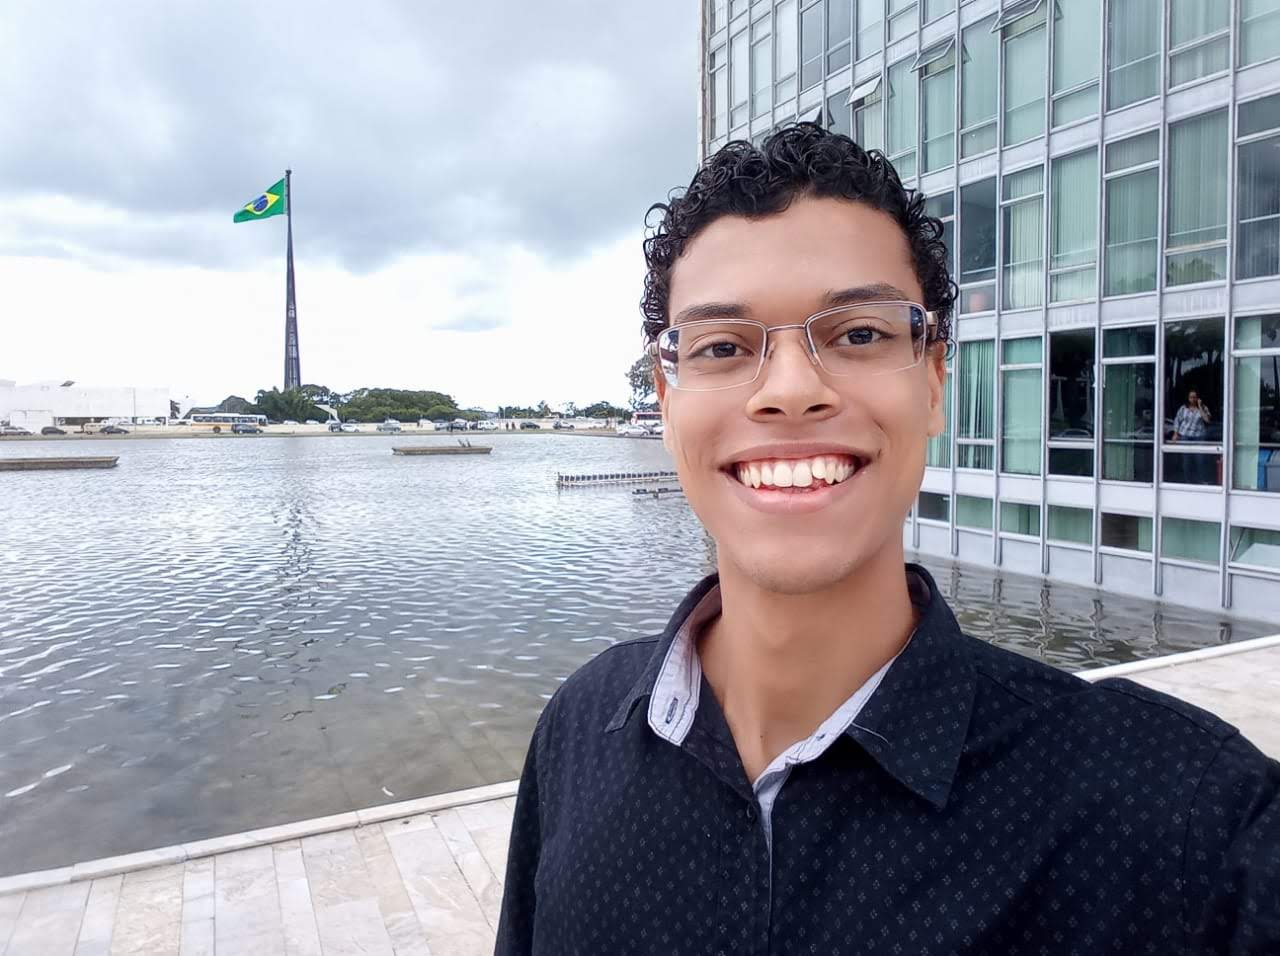
\includegraphics[width=\linewidth]{resources/perfil.jpeg}	%trimming relative to image size

%---------------------------------------------------------------------------------------
%	META SKILLS
%----------------------------------------------------------------------------------------
	\fcolorbox{white}{white}{\begin{minipage}[c][1.0cm][c]{1\mpwidth}
		\LARGE{\textbf{\textcolor{maincol}{Matheus Cardoso}}} \\[2pt]
		\normalsize{ \textcolor{maincol} {Computer Scientist (B. Sc.)} }
\end{minipage}}

\cvsection{Contato}

% \icontext{MapMarker}{16}{Street name XX\\D-XXXXX Lorem}{black}\\[6pt]
% \icontext{MobilePhone}{16}{+55 (61) 98264-5973}{black}\\[3pt]
\iconemail{Envelope}{16}{cardosaum@pm.me}{cardosaum@pm.me}{black}\\[3pt]
% \iconhref{Home}{16}{XXX.XXX-XXXX.XX}{http://XXX-XXX.XXX.XX}{black}\\[6pt]
\iconhref{Github}{16}{cardosaum}{https://www.github.com/cardosaum}{black}\\[3pt]
\iconhref{Linkedin}{16}{matheus-c-souza}{https://www.linkedin.com/in/matheus-c-souza}{black}\\[3pt]
\iconhref{Home}{16}{mcscv.netlify.com}{https://www.linkedin.com/in/matheus-c-souza}{black}\\[3pt]
% \iconhref{Xing}{16}{xing.com/user\_name}{https://www.xing.com/profile/User_Name}{black}\\


% \icontext{CaretRight}{12}{05.03.1999 in São Paulo}{black}\\[6pt]
% \icontext{CaretRight}{12}{Brazilian}{black}\\[6pt]
% \icontext{CaretRight}{12}{Unmarried}{black}\\[6pt]


%%%%%%%%
\cvsectionskill{Habilidades}

%%%%
\cvsectionsmall{Linguagens de\\ Programação}

\cvskill{Python} {3+ yrs.} {0.6}

\cvskill{Shell Scripting} {3+ yrs.} {0.6}

\cvskill{R} {1.5+ yrs.} {0.30}

\cvskill{C/C++} {1+ yrs.} {0.20}

\cvskill{SQL} {6+ mos.} {0.10}

\cvskill{Java} {6+ mos.} {0.10}

\cvskill{Rust} {6+ mos.} {0.10}

\cvskill{Javascript} {6+ mos.} {0.10}

\cvskill{RISC-V Assembly} {6+ mos.} {0.10}
%%%%

%%%%
\cvsectionsmall{Tecnologias}

\cvskill{HTML/CSS} {2.5+ yrs.} {0.50}

\cvskill{Git} {2.5+ yrs.} {0.50}

\cvskill{\LaTeX} {1.5+ yrs.} {0.30}
\vfill\null
%%%%

%%%%
\cvsectionsmall{Frameworks}

\cvskill{Biopython} {2.5+ yrs.} {0.50}

\cvskill{Tidyverse} {1.5+ yrs.} {0.30}

\cvskill{Tidymodels} {1.5+ yrs.} {0.30}

\cvskill{Numpy} {6+ mos.} {0.10}

\cvskill{Pandas} {6+ mos.} {0.10}

\cvskill{Django} {6- mos.} {0.06}
%%%%


%%%%
\cvsectionsmall{Áreas de experiência}

\cvskill{Administração de \newline Sistemas} {3+ yrs.} {0.6}

\cvskill{Bioinformática} {2.5+ yrs.} {0.5}

\cvskill{Ciência de Dados} {2+ yrs.} {0.4}

\cvskill{Sistemas Embarcados} {6+ mos.} {0.10}
%%%%


%%%%
\cvsectionsmall{Idiomas}

\cvskill{Português} {Nativo} {1}

\cvskill{Inglês} {B2} {0.66}

\cvskill{Espanhol} {B1} {0.50}
%%%%

%%%%%%%%

% \newpage
% %---------------------------------------------------------------------------------------
% %	EDUCATION
% %----------------------------------------------------------------------------------------
% \cvsection{Education}

% \cvmetaevent
% {01/2021 - Present}
% {Computer Science (B.Sc.)}
% {University of Brasília - UnB}

% \cvmetaevent
% {01/2020 - 12/2020}
% {Computer Science (B.Sc.)}
% {Federal University of Rio de Janeiro - UFRJ}
% {\footnotesize Note: Opted to change university due to COVID pandemic}

% \cvmetaevent
% {01/2019 - 12/2019}
% {Biotechnology (B.Sc.)}
% {University of Brasília - UnB}
% {\footnotesize Note: Opted to change university due to preference for programming}



% \cvsection{Projects}

% 	\href{https://github.com/cardosaum/attila}{\textbf{Attila}}\\ AutomaTed Tool For Immunoglobulin Analysis, A software to assess monoclonal antibody enrichment.\\

% 	\href{https://github.com/cardosaum/isc-lolo-game}{\textbf{The Adventures of Lolo}}\\ Remake of the game \textit{The Adventures of Lolo} in RISC-V assembly.\\

% 	\href{https://github.com/cardosaum/ufrj-comp1-senha}{\textbf{Mastermind}}\\ Remake of the game \textit{Mastermind} in C.\\


\cvsection{Interesses}

\icontext{CaretRight}{12}{Bioinformática/\\Biologia Computacional}{black}\\[6pt]
\icontext{CaretRight}{12}{Inteligência Artificial}{black}\\[6pt]
\icontext{CaretRight}{12}{Enovelamento de Proteínas}{black}\\[6pt]
\icontext{CaretRight}{12}{Projetos de código aberto}{black}\\[6pt]
\icontext{CaretRight}{12}{Sistemas Embarcados}{black}\\[6pt]

% \vfill
% \mbox{}
% \vfill
% \mbox{}
% \vfill
% \mbox{}
% \vfill
% \mbox{}
% \vfill
% \mbox{}
% \vfill
% \mbox{}
% \vfill
% \mbox{}
% \vfill
% \mbox{}
% \vfill
% \mbox{}
% \vfill
% \mbox{}
% \vfill
% \mbox{}
% \vfill
% \mbox{}
% \vfill
% \mbox{}


% \cvqrcode{0.3}

\end{leftcolumn}
\begin{rightcolumn}
%---------------------------------------------------------------------------------------
%	TITLE  HEADER
%----------------------------------------------------------------------------------------


%---------------------------------------------------------------------------------------
%	PROFILE
%----------------------------------------------------------------------------------------
\cvsection{Biografia}
\vspace{4pt}

\cvtext{

  Estudante de Ciências da Computação, trabalha com análise de dados na área de genômica e proteômica, desenvolvendo um software que gera, automaticamente, estatísticas sobre anticorpos monoclonais enriquecidos. Seu trabalho envolve principalmente técnicas de aprendizado de máquina, mineração, análise e visualização de dados. Como resultado, além de trabalhar na área de ciências da computação, também possui um grande foco em ciências biológicas e de dados.\\[-8pt]

  Em seu tempo livre, ele também tem contribuído para projetos de código aberto; Abrangendo desde frameworks para ciência de dados (\href{https://pandas.pydata.org/}{Pandas}) a softwares educacionais para aprendizado (\href{https://apps.ankiweb.net/}{Anki}) e programas de produtividade (\href{https://github.com/hrkfdn/ncspot/}{ncspot}, \href{https://github.com/Airblader/unclutter-xfixes/issues/67}{unclutter} and \href{https://github.com/Cardosaum/hacksaw/}{hacksaw}).

  % \Blindtext[1]


}


%---------------------------------------------------------------------------------------
%	WORK EXPERIENCE
%----------------------------------------------------------------------------------------

\vspace{10pt}
\cvsection{Educação}
\vspace{4pt}


\cvevent
{03/2021 - presente}
	{Bacharelado em Ciências da Computação}
	{Universidade de Brasília - UnB}
	{Graduação ainda em curso. Sou aluno de destaque da turma, com grandes chances de formar com honras.\\[5]Rendimento Acadêmico: 5/5}
	% {I don't have much to say yet.\\[5]GPA: 4.8/5}
	\vfill\null


\cvevent
{01/2020 - 03/2021}
	{Bacharelado em Ciências da Computação}
	{Universidade Federal do Rio de Janeiro - UFRJ}
	{Devido a pandemia, optei por me mudar do Rio de Janeiro de volta para Brasília.\\[5]Rendimento Acadêmico: 2.9/5}
	\vfill\null

	
\cvevent
{01/2019 - 12/2019}
	{Bacharelado em Biotecnologia}
	{Universidade de Brasília - UnB}
	{Eu tive a oportunidade de estagiar no laboratório de Bioinformática e Imunologia do laboratório da UnB, onde contribuí, e ainda contribuo, para o desenvolvimento de um software para analisar o enriquecimento de anticorpos monoclonais. Lá eu descobri que, mais do que pesquisar, eu gostava de programar. Dessa forma, optei por mudar de curso.\\[5]Rendimento Acadêmico: 4.8/5}
	\vfill\null


\cvsection{Projetos}

\cvevent
{01/2019 - presente}
	{\href{https://github.com/cardosaum/attila}{\textbf{ATTILA - AutomaTed Tool For Immunoglobulin}}}
	{Universidade de Brasília - UnB}
	{ATTILA é um programa de código aberto que analisa bibliotecas de phage display de forma a avaliar o enriquecimento de anticorpos monoclonais. Fazendo isso, o software é capaz de predizer quais anticorpos podem se ligar de forma mais efetiva a moléculas alvo. Dessa forma, o ATTILA se torna uma ferramenta útil a cientistas que trabalham no desenvolvimento de vacinas.} \vfill\null

  \cvevent {06/2021 - presente}
  {\href{https://github.com/cardosaum/cdr3-parser}{\textbf{cdr3-parser}}}
  {Universidade de Brasília - UnB}
  {\textbf{cdr3-parser} é um programa de linha de comando escrito em \texttt{Rust} para converter arquivos intermediários gerados pelo ATTILA em arquivos \texttt{csv} com estatísticas sobre as regiões VH-CDR3 presentes no arquivo inicial. \textbf{cdr3-parser} faz uso das características de paralelismo seguro proporcionadas pela linguagem \texttt{Rust} para analisar o arquivo inicial da forma mais eficiente possível, usando todas as threads disponíveis do servidor existente no laboratório de Bioinformática da UnB.} \vfill\null


\cvevent
{03/2021 - 05/2021}
	{\href{https://github.com/cardosaum/isc-lolo-game}{\textbf{The Adventures of Lolo}}}
    {Universidade de Brasília - UnB}
	{Recriação do jogo \textit{The Adventures of Lolo} em \texttt{RISC-V Assembly}.}
	\vfill\null


\cvevent
{02/2021 - 03/2021}
	{\href{https://github.com/cardosaum/ufrj-comp1-senha}{\textbf{Mastermind}}}
	{Universidade Federal do Rio de Janeiro - UFRJ}
	{Recriação do jogo \textit{Mastermind} em \texttt{C}.}
  \vfill\null

\cvevent
{08/2020}
	{\href{https://cardosaum.shinyapps.io/Matheus-Cardoso-DDP-JHU-Week4}{\textbf{Brazilian Students' Performance on ENEM}}}
	{Johns Hopkins Bloomberg School of Public Health}
	{Um projeto de visualização de dados mostrando a performance dos estudantes brasileiros que concorreram ao curso de Bacharelado em Ciências da Computação da Universidade de São Paulo, uma das melhores do país.}
  \vfill\null

\cvevent
{08/2020}
	{\href{https://cardosaum.shinyapps.io/WordPredictor_Final_Project_JHU_Matheus_C}{\textbf{Word Predictor Model}}}
	{Johns Hopkins Bloomberg School of Public Health}
	{Um aplicativo web que usa técnicas de aprendizado de máquina para predizer a próxima palavra em uma frase.}
  \vfill\null


\cvsection{Prêmios \& Certificados}

\cvevent
{01/2020 - 09/2020}
	{\href{https://www.coursera.org/account/accomplishments/specialization/certificate/JTYMU3V78XWZ}{\textbf{Especialização em Ciência de Dados}}}
	{Johns Hopkins Bloomberg School of Public Health}
	{}
	\vfill\null

\cvevent
{2020}
	{\textbf{Hackathon de Bioinformática de Copenhague}}
	{BioLib}
	{Ganhador do Hackathon na modalidade \textit{``Predição de Patogenicidade''}.}
	\vfill\null

\cvevent
{2019}
	{\href{https://talentouniversitario.capes.gov.br/#!/index}{\textbf{Prêmio Capes Talento Universitário}}}
	{CAPES}
	{Premiado pelo Ministério da Eduação, por meio da CAPES, como um dos 1000 calouros mais talentosos do país.}
	\vfill\null

\cvevent
{2019}
	{Hackathon NASA Space Apps BSB}
	{NASA}
	{Premiado como 5º colocado, em mais de 60 times, na fase regional do Hackathon no Brasil.}
	\vfill\null


% \cvsection{Service}

% \cvevent
% {2019}
% 	{CPA}
% 	{NASA}
% 	{Awarded as 5th out of 60+ teams in the Brazil's Midwest regional phase.}
% 	\vfill\null

% \cvevent
% {03/2020 - 09/2020}
% 	{\href{https://www.coursera.org/account/accomplishments/specialization/certificate/JTYMU3V78XWZ}{\textbf{Data Science Specialization}}}
% 	{Johns Hopkins Bloomberg School of Public Health}
% 	{}
% 	\vfill\null



% \cvsection{Publications}

% \item Author, G. \& Author, P. \&  Author G. (2020). "This is the title of the publication". In: \textit{Proceedings of the 28th Conference on Lipsum (LIPSUM)}, Lipsum, June 12-17, 2020.
% \item Author, G. \& Author, P. \&  Author G. (2020). "This is the title of the publication". In: \textit{Proceedings of the 28th Conference on Lipsum (LIPSUM)}, Lipsum, June 12-17, 2020.
% \item Author, G. \& Author, P. \&  Author G. (2020). "This is the title of the publication". In: \textit{Proceedings of the 28th Conference on Lipsum (LIPSUM)}, Lipsum, June 12-17, 2020.
% \end{itemize}

% % hofixes to create fake-space to ensure the whole height is used
\mbox{}
\vfill
\mbox{}
\vfill
\mbox{}
\vfill
\mbox{}
\vfill
\mbox{}
\vfill
\mbox{}
\vfill
\mbox{}
\vfill
\mbox{}
\vfill
\mbox{}
\vfill
\mbox{}
\vfill
\mbox{}


São Paulo, \today \hspace{1cm} \hrulefill

\hspace*{30mm}\phantom{Lorem, \today }Matheus Cardoso de Souza

\end{rightcolumn}
\end{paracol}


\end{document}
